\newcommand{\pluginName}{Yahoo! Finance Integration}
\newcommand{\pluginVersion}{1.0}

\input{../../../DocumentationTemplate/TemplateL3}

\begin{document}

\PluginTitle{\pluginName}{\pluginVersion}

\section{Introduction}
Thee \textbf{\pluginName}  plug-in allows Fairmat to use market data published on the Yahoo! Finance service to calibrate equity models and to retrieve historical prices series. 
Currently the the models which can benefit from this data providers the Geometric Brownian Motion (historical series calibration) and the Historical Simulator plug-ins which implements bootstrapping.



\section{How to use the \pluginName { } plug-in}
\begin{itemize}
\item Choose \textbf{\pluginName} in Settings / Fairmat Preferences / Market Data Provider

\item Connect the project underlying asset to Market Data: when a data provider is present the \textbf{Data Source} tab is available on the stochastic processes editing forms. 
This tab is used to bind the process to the market and to specify how the process must be calibrated. Relevant fields are the ticker name, in this case the equity or the index, the reference market
and how the process must be calibrated (Calibration Options).
\begin{figure}[h]
\begin{center}
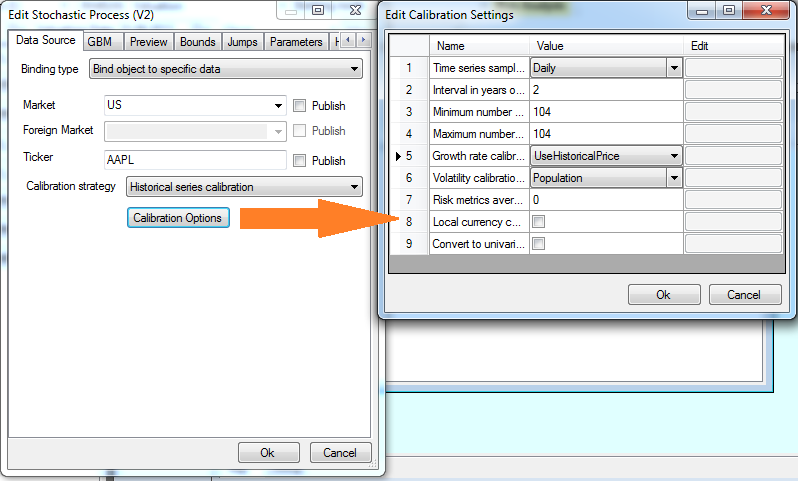
\includegraphics[width=0.7\textwidth]{./Figures/DataSourcesTab.png}
\caption{Data Sources Tab allows to specify how the stochastic process is connected to market data.}
\label{fig.DataSourceTab}
\end{center}
\end{figure}
\end{itemize}



\end{document}


